\chapter{Explainability}

\textbf{Interpretability} (or \textbf{explainability}) is the degree to which a human can understand the cause of a decision. The higher the interpretability of a model, the easier it is for a person to understand why certain decisions or precisions have been made. Interpretability can be used not only to understand why a model gives a specific prediction, but also to highlight biases in the model or the data.

A \textbf{black box} is a model whose internals are either unknown to the observer, or they are known but uninterpretable by humans. Some examples of black box models are deep neural networks, support vector machines, and ensemble methods. Other models are instead interpretable by design, such as decision trees, linear regression, logistic regression, and rule-based models.

Machine learning interpretability can be classified according to various criteria:
\begin{itemize}
    \item \textbf{Intrinsic or post-hoc}: intrinsic interpretability refers to models that are considered interpretable because of their simple structure, such as short decision trees or sparse linear models. Post-hoc interpretability refers to the application of interpretation methods after model training. Post.hoc methods can also be applied to intrinsecally interpretable models.
    
    \item \textbf{Model-specific or model-agnostic}: model-specific interpretation methods are limited to specific model classes (e.g., the interpretation of regression weights in a linear model is model-specific). Model-agnostic methods can be applied on any machine learning model after the model has been trained. The latter work by analyzing the input and output pairs, since bydefinition they do not have access to the model internals.
    
    \item \textbf{Local or global}: global methods explain the entire method's behaviour, while local ones explain the prediction of single instances.
\end{itemize}
Intrinsic interpretability methods are always both global and model specific.

Explanations are provided in different formats depending on the input data type: tabular data uses decision trees, feature importance; image data uses saliency maps, contingency maps; text data uses sentence higlighting, attention-based methods. For all of them, prototypes and counter-exemplars can be used, as well.

\begin{figure}[ht]
    \centering
    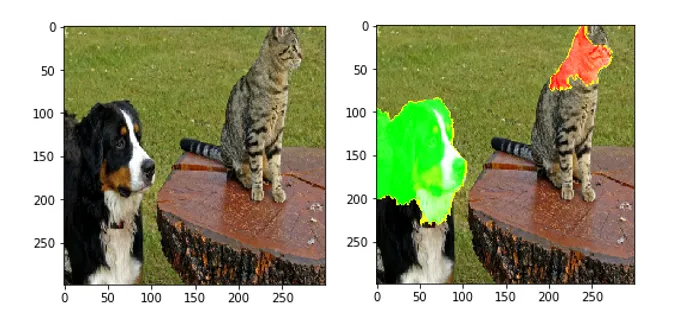
\includegraphics[width=0.75\textwidth]{img/saliency_map_dog_cat.png}
    \caption{Saliency map for a photo of a cat and a dog. The areas highlighted in green represent those which contribute positively to classifying it as "Bernese dog", while the red areas are those which contribute negatively.}
\end{figure}
\begin{figure}[ht]
    \centering
    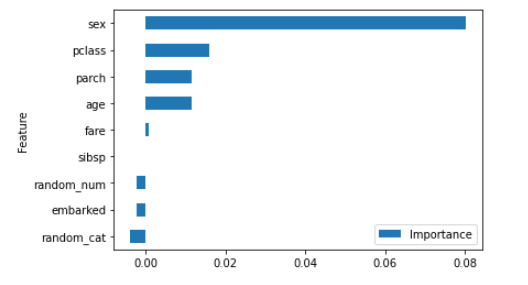
\includegraphics[width=0.70\textwidth]{img/feature_importance.png}
    \caption{A plot showing feature importance for a dataset. A positive importance means the feature strongly contributes to the prediction, while a negative importance means the feature is negatively correlated with the prediction.}
\end{figure}

\section{Explanation Methods}

\subsection{TREPAN}

TREPAN is a global explainer first developed to extract symbolic representations from trained neural networks (although they are usable on any kind of black box model). TREPAN queries a neural network and builds a decision tree that approximates the network's behaviour using $m$-of-$n$ rules: $m$-of-$n$ expressions are Boolean expressions that are specified by an integer threshold $m$, and a set of $n$ Boolean conditions, and is satisfied if at least $m$ of its $n$ conditions are satisfied. A limitation of regular decision trees is that at lower depths, splits are less significative since they are based on few training instances. TREPAN instead can select as many instances as it wants to build a split condition rule. It learns to predict the label returned by the black box, not the original one.

When selecting a split at a given node, the oracle is given the list of all the previously selected splits on the path from the root to that node. This information is needed to restrict the feature values to consider to build the rule. 

\subsection{LIME}

LIME (Local Interpretable Model-agnostic Explanations) is a local explainer which implements surrogate models (a logistic regressor, usually with LASSO or Ridge regularization), trained to approximate the predictions of underlying black box model. LIME works by perturbing the data instance, generating a new dataset composed of perturbed instances and their corresponding predictions by the black box model. An interpretable model is trained on this new dataset, weighted by the proximity of the sampled instances to the instance of interest. This surrogate should be a good approximation of the original model locally, but not globally: this kind of ``accuracy'' is called \textbf{local fidelity}.

When using tabular data, instances are perturbed by changing values of the features, drawing from a normal distribution with mean and standard deviation taken from the feature itself. Each feature will be assigned an importance, describing how much each of them contributes (positively or negatively) to the prediction. For image or text data, the solution is to exclude certain pixels or words. Specifically, images are transformed into vectors of interpretable superpixels expressing presence or absence; a synthetic neighborhood is obtained perturbing these vectors, and the surrogate ends up assigning weights to each superpixel. This is done because perturbing single pixels is not enough to change predictions by much. 

\subsection{LORE}

LORE (LOcal Rule-based Explainer) extends LIME using a decision tree as a surrogate, and generating synthetic instances using a genetic procedure that takes into account for instances with the same labels and those with different ones. Local explanations are expressed in the form of pairs, composed by a logic rule, describing a path in the decision tree that explains why the instance has been classified as such, and a set of \textbf{counterfacual rules}, explaining which conditions should be changed to obtain a different prediciton. It can be generalized to work on text and image data, using the same data representation as LIME.

\subsection{SHAP}

\textbf{Shapley values} are a method from coalitional game theory which can be used to find how to evenly distribute the ``payout'' (the prediction) across the ``players'' (the features). The goal is to explain the difference between the prediction and the average prediction for all instances. The Shapley value is the average marginal contribution of a feature across all possible coalitions. A coalition between features is simulated by randomly selecting another instance from the dataset and using its values for the features not in the coalition, obtaining a new instance. Since this procedure is highly computationally expensive, so an alternative is to compute contributions for only a few samples of the possible coalitions.

SHAP (SHapley Additive exPlanations) is a model-agnostic method based on Shapley values. Its goal is to explain the prediction of a given instance by compuiting the contribution of each feature to the prediction calculating their Shapley values. Players can also be groups of features instead of individual ones. In SHAP, Shapley value explanation is represented as an additive feature attribution method, a linear model:
\begin{equation*}
    g(z') = \phi_0 + \sum_{i=1}^M \phi_i z_i'
\end{equation*}
where $g$ is the explanation model, $z'$ the coalition vector, $M$ the maximum coalition size, and $\phi_i$ is the Shapley value of feature $i$.

\subsection{Integrated Gradients}

Integrated gradients is a method that computes the gradients of all the points between the input instance and the baseline input (for images, this could be a black image; for text, the zero embedding vector): the intgrated gradients are the cumulation of these gradients. The result can be visualized using the appropriate format (e.g., saliency maps for images).

\subsection{Instance-Based Explanations}

Instance-based explanation methods select particular instances or generate synthetic instances to explain black box model behaviour. They are mainly local explainers. These methods make sense if the input can be represented in a human understandable way, such as tabular data with few features, images, or short text. Instance-based methods can be divided mainly into two groups:
\begin{itemize}
    \item \textbf{Prototypes}: a selection of representative instances with the same class as the instance under analysis, among which we can distinguish \textbf{criticisms} (instances that are not well represented  by prototypes), \textbf{influential instances} (training points that were the most influential for the training of the black-box model or for the prediction);
    
    \item \textbf{Counterfactuals}: a selection of represetative instances with a different class than the instance under analysis. A counterfactual explanation represents the smallest change to the feature values that changes the prediction to a specific class (or simply the other class, in a binary task).
\end{itemize}

\subsubsection{Generating Counterfactuals}

A naive approach is to use trial-and-error, randomly changing feature values of the instance and stopping when the desired output is obtained. A more sophisticated approach is to define a loss function that considers the instance of interest, the counterfactual, and the desired outcome: the counterfactual explanation that minimizes this loss can be found using an optimization algorithm. There are many different methods, each using a different loss function and optimization algorithm.

One such method defines the loss as:
\begin{equation*}
    L(x,x',y',\lambda) = \lambda \cdot (\hat{f}(x') - y')^2 + d(x,x')
\end{equation*}
The first term is the squared difference between the prediction of the counterfactual $x'$ and the desired outcome $y'$, and the second term is the distance between the instance under analysis and the counterfactual, defined as a Manhattan distance weighted by the median absolute devation (MAD). $\lambda$ is a regularization term. By minimizing this loss, we find the closest counterfactual to the instance that changes the prediction. Instead of selecting a specific value for $\lambda$, a tolerance can be set instead, such that the following constraint must be satisfied:
\begin{equation*}
    |\hat{f}(x') - y'| \leq \epsilon
\end{equation*}
The steps taken to generate counterfactuals are:
\begin{itemize}
    \item An instance $x$, a desired outcome $y'$, a tolerance $\epsilon$, and a regularization term $\lambda$ are chosen;
    \item A random instance is sampled as initial counterfactual;
    \item The loss is optiimzed, using that counterfactual as the starting point;
    \item While $|\cap{f}(x') - y'| > \epsilon$, $\lambda$ is increased and the loss is optimized again. The counterfactual that minimizes the loss is returned.
    \item Steps 2-4 are repeated and a list of counterfactuals is returned (or only the one that minimizes the loss).
\end{itemize}

Another method, called \textbf{DICE} (\textbf{Diverse Counterfactual Explanations}), solves an optimization problem with penalization terms that ensure plausibility by similarity and diversity; it returns a set of $k$ plausible and different counterfactuals are calculated as:
\begin{equation*}
    C(x) = \arg \min_{c_1, \dots, c_k} \dfrac{1}{k} \sum_{i=1}^k L(f(c_i), y') + \dfrac{\lambda_1}{k} \sum_{i=1}^k d(c_i, x) - \lambda_2 \textit{dpp-diversity}(c_1, \dots, c_k)
\end{equation*}
where \textit{dpp-diversity} is ``diversity via determinantal point processes'', a measure of diversity between the counterfactuals. 

Finally, counterfactuals can be found using \textbf{heuristic strategies}. These strategies are usually more efficient than optimization algorithms, but do not necessarily find solutions that are optimal. The search strategy is designed so that at each iteration, $x'$ is updated with the objective of minimizing a cost function.

An example of a heuristic strategy is \textbf{GSG} (\textbf{Growing Spheres Generation}), which relies on a generative approach growing a sphere of syntetic instances around $x$ to find the closest counterfactual: it ignores the direction towards which the closest classification boundary might be, so the solution is not always optimal. The algorithm generates observations in spherical layers around the instance, until a potential counterfactual is found.

Another example is \textbf{NNCE} (\textbf{Nearest-Neighbor Counterfactual Explainer}), which selects counterfactuals as the instances $x'$ most similar to $x$ and with a different label, using a nearest-neighbor search. Candidate counterfactuals are sorted with respect to the distance between $x$, and the $k$ most similar ones are selected.

Finally, \textbf{CBCE} (\textbf{Case-Based Counterfactual Explainer}) is a refinement of NNCE, which adopts the notion of \textbf{explanation case} ($xc$). Given a dataset $X$, an $xc$ is a couple of instances $(x,x')$ such that $x$ and $x'$ are the two most similar instances in $X$, and they have different labels.